\documentclass[12pt,a4paper,twoside,openright]{report}
\let\openright=\cleardoublepage



%%% Choose a language %%%

\newif\ifEN
\ENtrue   % uncomment this for english
%\ENfalse   % uncomment this for czech

%%% Configuration of the title page %%%

\def\ThesisTitleStyle{mff} % MFF style
%\def\ThesisTitleStyle{cuni} % uncomment for old-style with cuni.cz logo
%\def\ThesisTitleStyle{natur} % uncomment for nature faculty logo

\def\UKFaculty{Faculty of Mathematics and Physics}
%\def\UKFaculty{Faculty of Science}

\def\UKName{Charles University in Prague} % this is not used in the "mff" style

% Thesis type names, as used in several places in the title
\def\ThesisTypeTitle{\ifEN BACHELOR THESIS \else BAKALÁŘSKÁ PRÁCE \fi}
%\def\ThesisTypeTitle{\ifEN MASTER THESIS \else DIPLOMOVÁ PRÁCE \fi}
%\def\ThesisTypeTitle{\ifEN RIGOROUS THESIS \else RIGORÓZNÍ PRÁCE \fi}
%\def\ThesisTypeTitle{\ifEN DOCTORAL THESIS \else DISERTAČNÍ PRÁCE \fi}
\def\ThesisGenitive{\ifEN bachelor \else bakalářské \fi}
%\def\ThesisGenitive{\ifEN master \else diplomové \fi}
%\def\ThesisGenitive{\ifEN rigorous \else rigorózní \fi}
%\def\ThesisGenitive{\ifEN doctoral \else disertační \fi}
\def\ThesisAccusative{\ifEN bachelor \else bakalářskou \fi}
%\def\ThesisAccusative{\ifEN master \else diplomovou \fi}
%\def\ThesisAccusative{\ifEN rigorous \else rigorózní \fi}
%\def\ThesisAccusative{\ifEN doctoral \else disertační \fi}



%%% Fill in your details %%%

% (Note: \xxx is a "ToDo label" which makes the unfilled visible. Remove it.)
\def\ThesisTitle{TaleCraft — Framework for 2D point-and-click adventure games}
\def\ThesisAuthor{Alžbeta Kulichová}
\def\YearSubmitted{2025}

% department assigned to the thesis
\def\Department{Department of Distributed and Dependable Systems}
% Is it a department (katedra), or an institute (ústav)?
\def\DeptType{Department}

\def\Supervisor{Mgr. Pavel Ježek, Ph.D.}
\def\SupervisorsDepartment{Department of Distributed and Dependable Systems}

% Study programme and specialization
\def\StudyProgramme{Computer Science}
\def\StudyBranch{Computer Graphics, Vision and Game Development }

\def\Dedication{
I would like to thank my supervisor Mgr. Pavel Ježek, Ph.D. for guidance he gave me during the writing of this thesis. I am also grateful to my family and friends for supporting me throughout my studies. Lastly, special thanks goes to my loving boyfriend, who was there for me even during the most difficult moments and without whom I would not be the person I am today.}

\def\AbstractEN{This thesis implements a C\# framework for 2D point-and-click adventure games built in the Unity engine. While similar tools exist in the Unity Asset store, point-and-click adventure games often rely on custom-built solutions, and there is still value in creating a lightweight, adaptable framework that can serve as both a development aid and a learning resource. It allows game developers to streamline the development of fundamental gameplay systems typical of the genre. At the same time, it offers flexibility and customizable components to accommodate a wide range of artistic styles and narrative structures. The framework provides core mechanics commonly found in point-and-click adventures such as a walking system, dialogue system, inventory system, and more. To showcase how the framework works in practice, a simple prototype game was created using its features. While the framework is not fully complete and does not include every mechanic a finished game might need, it provides a solid foundation and a starting point for future improvements and additional functionality.}

\def\AbstractCS{Tato práce implementuje C\# framework pro 2D point-and-click adventury v Unity enginu. Zatímco podobné nástroje existují v obchodě Unity Asset, dobrodružné hry typu point-and-click často spoléhají na řešení vytvořená na míru a stále je užitečné vytvořit lehký, přizpůsobivý framework, který může sloužit jako vývojová pomůcka i jako zdroj výuky. Umožňuje vývojářům her zefektivnit vývoj základních herních systémů typických pro tento žánr. Zároveň nabízí flexibilitu a přizpůsobitelné komponenty, aby vyhovovaly široké škále uměleckých stylů a narativních struktur. Framewok poskytuje základní mechaniky, které se běžně vyskytují v dobrodružstvích typu point-and-click, jako je systém pohybu, systém dialogů, systém inventáře a další. Abychom předvedli, jak framework funguje v praxi, byl vytvořen jednoduchý prototyp hry využívající jeho funkce. Přestože framework není zcela kompletní a nezahrnuje všechny mechaniky, které by hotová hra mohla potřebovat, poskytuje pevný základ a výchozí bod pro budoucí vylepšení a další funkce.}

% 3 to 5 keywords (recommended), each enclosed in curly braces.
% Keywords are useful for indexing and searching for the theses by topic.
\def\Keywords{
{Unity} {framework} {2D game} {point-and-click adventure game}
}

% If your abstracts are long and do not fit in the infopage, you can make the
% fonts a bit smaller by this setting. (Also, you should try to compress your abstract more.)
% Alternatively, consider increasing the size of the page by uncommenting the
% geometry modification in thesis.tex.
\def\InfoPageFont{}
%\def\InfoPageFont{\small}  %uncomment to decrease font size

\ifEN\relax\else
% If you are writing a czech thesis, you additionally need to fill in the
% english translation of the metadata here!
\def\ThesisTitleEN{TaleCraft — Framework for 2D point-and-click adventure games}
\def\DepartmentEN{Department of Distributed and Dependable Systems}
\def\DeptTypeEN{Department}
\def\SupervisorsDepartmentEN{Department of Distributed and Dependable Systems}
\def\StudyProgrammeEN{Computer Science}
\def\StudyBranchEN{Computer Graphics and Game Engineering}
\def\KeywordsEN{{Unity} {framework} {2D game} {point-and-click adventure game}
}
\fi


\usepackage[a-2u]{pdfx}

\ifEN\else\usepackage[czech,shorthands=off]{babel}\fi
\usepackage[utf8]{inputenc}
\usepackage[T1]{fontenc}

% See https://en.wikipedia.org/wiki/Canons_of_page_construction before
% modifying the size of printable area. LaTeX defaults are great.
% If you feel it would help anything, you can enlarge the printable area a bit:
%\usepackage[textwidth=390pt,textheight=630pt]{geometry}
% The official recommendation expands the area quite a bit (looks pretty harsh):
%\usepackage[textwidth=145mm,textheight=247mm]{geometry}

%%% FONTS %%%
\usepackage{lmodern} % TeX "original" (this sets up the latin mono)

% Optionally choose an override for the main font for typesetting:
\usepackage[mono=false]{libertinus} % popular for comp-sci (ACM uses this)
%\usepackage{tgschola} % Schoolbook-like (gives a bit of historic feel)
%\usepackage[scale=0.96]{tgpagella} % Palladio-like (popular in formal logic).
% IBM Plex font suite is nice but requires us to fine-tune the sizes, also note
% that it does not directly support small caps (\textsc) and requires lualatex:
%\usepackage[usefilenames,RM={Scale=0.88},SS={Scale=0.88},SScon={Scale=0.88},TT={Scale=0.88},DefaultFeatures={Ligatures=Common}]{plex-otf}

% Optionally, choose a custom sans-serif fonts (e.g. for figures and tables).
% Default sans-serif font is usually Latin Modern Sans. Some font packages
% (e.g. libertinus) replace that with a better matching sans-serif font.
%\usepackage{tgheros} % recommended and very readable (Helvetica-like)
%\usepackage{FiraSans} % looks great
% DO NOT typeset the main text in sans-serif font!
% The serifs make the text easily readable on the paper.


% IMPORTANT FONT NOTE: Some fonts require additional PDF/A conversion using
% the pdfa.sh script. These currently include only 'tgpagella'; but various
% other fonts from the texlive distribution need that too (mainly the Droid
% font family).


% some useful packages
\usepackage{microtype}
\usepackage{amsmath,amsfonts,amsthm,bm}
\usepackage{graphicx}
\usepackage{xcolor}
\usepackage{booktabs}
\usepackage{caption}
\usepackage{floatrow}

% load bibliography tools
\usepackage[backend=bibtex,natbib,style=numeric,sorting=none]{biblatex}
% alternative with alphanumeric citations (more informative than numbers):
%\usepackage[backend=bibtex,natbib,style=alphabetic]{biblatex}
%
% alternatives that conform to iso690
% (iso690 is not formally required on MFF, but may help elsewhere):
%\usepackage[backend=bibtex,natbib,style=iso-numeric,sorting=none]{biblatex}
%\usepackage[backend=bibtex,natbib,style=iso-alphabetic]{biblatex}
%
% additional option choices:
%  - add `giveninits=true` to typeset "E. A. Poe" instead of full Edgar Allan
%  - `terseinits=true` additionaly shortens it to nature-like "Poe EA"
%  - add `maxnames=10` to limit (or loosen) the maximum number of authors in
%    bibliography entry before shortening to `et al.` (useful when referring to
%    book collections that may have hundreds of authors)
%  - for additional flexibility (e.g. multiple reference sections, etc.),
%    remove `backend=bibtex` and compile with `biber` instead of `bibtex` (see
%    Makefile)
%  - `sorting=none` causes the bibliography list to be ordered by the order of
%    citation as they appear in the text, which is usually the desired behavior
%    with numeric citations. Additionally you can use a style like
%    `numeric-comp` that compresses the long lists of citations such as
%    [1,2,3,4,5,6,7,8] to simpler [1--8]. This is especially useful if you plan
%    to add tremendous amounts of citations, as usual in life sciences and
%    bioinformatics.
%  - if you don't like the "In:" appearing in the bibliography, use the
%    extended style (`ext-numeric` or `ext-alphabetic`), and add option
%    `articlein=false`.
%
% possibly reverse the names of the authors with the default styles:
%\DeclareNameAlias{default}{family-given}

% load the file with bibliography entries
\addbibresource{refs}

% remove this if you won't use fancy verbatim environments
\usepackage{fancyvrb}

% remove this if you won't typeset TikZ graphics
\usepackage{tikz}
\usetikzlibrary{positioning} %add libraries as needed (shapes, decorations, ...)

% remove this if you won't typeset any pseudocode
\usepackage{algpseudocode}
\usepackage{algorithm}

% remove this if you won't list any source code
\usepackage{listings}


\hypersetup{unicode}
\hypersetup{breaklinks=true}

\usepackage[noabbrev]{cleveref}

\input{todos} % remove this before compiling the final version


% use this for typesetting a chapter without a number, e.g. intro and outro
\def\chapwithtoc#1{\chapter*{#1}\addcontentsline{toc}{chapter}{#1}}

% If there is a line/figure overflowing into page margin, this will make the
% problem evident by drawing a thick black line at the overflowing spot. You
% should not disable this.
\overfullrule=3mm

% The maximum stretching of a space. Increasing this makes the text a bit more
% sloppy, but may prevent the overflows by moving words to next line.
\emergencystretch=1em

\ifEN
\theoremstyle{plain}
\newtheorem{thm}{Theorem}
\newtheorem{lemma}[thm]{Lemma}
\newtheorem{claim}[thm]{Claim}
\newtheorem{defn}{Definition}
\theoremstyle{remark}
\newtheorem*{cor}{Corollary}
\else
\theoremstyle{plain}
\newtheorem{thm}{Věta}
\newtheorem{lemma}{Lemma}
\newtheorem{claim}{Tvrzení}
\newtheorem{defn}{Definice}
\theoremstyle{remark}
\newtheorem*{cor}{Důsledek}
\fi

\newenvironment{myproof}{
  \par\medskip\noindent
  \textit{\ifEN Proof \else Důkaz \fi}.
}{
\newline
\rightline{$\qedsymbol$}
}

% real/natural numbers
\newcommand{\R}{\mathbb{R}}
\newcommand{\N}{\mathbb{N}}

% asymptotic complexity
\newcommand{\asy}[1]{\mathcal{O}(#1)}

% listings and default lstlisting config (remove if unused)
\DeclareNewFloatType{listing}{}
\floatsetup[listing]{style=ruled}

\DeclareCaptionStyle{thesis}{style=base,font={small,sf},labelfont=bf,labelsep=quad}
\captionsetup{style=thesis}
\captionsetup[algorithm]{style=thesis,singlelinecheck=off}
\captionsetup[listing]{style=thesis,singlelinecheck=off}

% Customization of algorithmic environment (comment style)
\renewcommand{\algorithmiccomment}[1]{\textcolor{black!25}{\dotfill\sffamily\itshape#1}}

% Uncomment for table captions on top. This is sometimes recommended by the
% style guide, and even required for some publication types.
%\floatsetup[table]{capposition=top}
%
% (Opinionated rant:) Captions on top are not "compatible" with the general
% guideline that the tables should be formatted to be quickly visually
% comprehensible and *beautiful* in general (like figures), and that the table
% "head" row (with column names) should alone communicate most of the content
% and interpretation of the table. If you just need to show a long boring list
% of numbers (because you have to), either put some effort into showing the
% data in an attractive figure-table, or move the data to an attachment and
% refer to it, so that the boredom does not impact the main text flow.
%
% You can make the top-captions look much less ugly by aligning the widths of
% the caption and the table, with setting `framefit=yes`, as shown below.  This
% additionally requires some extra markup in your {table} environments; see the
% comments in the example table in `ch2.tex` for details.
%\floatsetup[table]{capposition=top,framefit=yes}

\ifEN\floatname{listing}{Listing}
\else\floatname{listing}{Výpis kódu}\fi
\lstset{ % use this to define styling for any other language
  language=C++,
  tabsize=2,
  showstringspaces=false,
  basicstyle=\footnotesize\tt\color{black!75},
  identifierstyle=\bfseries\color{black},
  commentstyle=\color{green!50!black},
  stringstyle=\color{red!50!black},
  keywordstyle=\color{blue!75!black}}

% Czech versions of the used cleveref references (It's not as convenient as in
% English because of declension, cleveref is limited to sg/pl nominative. Use
% plain \ref to dodge that.)
\ifEN\relax\else
\crefname{chapter}{kapitola}{kapitoly}
\Crefname{chapter}{Kapitola}{Kapitoly}
\crefname{section}{sekce}{sekce}
\Crefname{section}{Sekce}{Sekce}
\crefname{subsection}{sekce}{sekce}
\Crefname{subsection}{Sekce}{Sekce}
\crefname{subsubsection}{sekce}{sekce}
\Crefname{subsubsection}{Sekce}{Sekce}
\crefname{figure}{obrázek}{obrázky}
\Crefname{figure}{Obrázek}{Obrázky}
\crefname{table}{tabulka}{tabulky}
\Crefname{table}{Tabulka}{Tabulky}
\crefname{listing}{výpis}{výpisy}
\Crefname{listing}{Výpis}{Výpisy}
\floatname{algorithm}{Algoritmus}
\crefname{algorithm}{algoritmus}{algoritmy}
\Crefname{algorithm}{Algoritmus}{Algoritmy}
\newcommand{\crefpairconjunction}{ a~}
\newcommand{\crefrangeconjunction}{ a~}
\fi
 % use this file for various custom definitions


\begin{document}

% the layout is mandatory, edit only in dire circumstances

\pagestyle{empty}
\hypersetup{pageanchor=false}
\begin{center}

% top part of the layout, this actually differs between faculties

\def\ThesisTitleXmff{%
  \ifEN
    \centerline{\mbox{\includegraphics[width=166mm]{img/logo-en.pdf}}}
  \else
    \centerline{\mbox{\includegraphics[width=166mm]{img/logo-cs.pdf}}}
  \fi
  \vspace{-8mm}\vfill%
  {\bf\Large\ThesisTypeTitle}
  \vfill%
  {\LARGE\ThesisAuthor}\par
  \vspace{15mm}%
  {\LARGE\bfseries\ThesisTitle}
  \vfill%
  \Department}
\def\ThesisTitleCuniLogo#1{%
  {\large\UKName\par\medskip\par\UKFaculty }
  \vfill%
  {\bf\Large\ThesisTypeTitle}
  \vfill%
  \includegraphics[width=70mm]{#1}
  \vfill%
  {\LARGE\ThesisAuthor}\par
  \vspace{15mm}%
  {\LARGE\bfseries\ThesisTitle}
  \vfill%
  \Department\par}
\def\ThesisTitleXcuni{\ThesisTitleCuniLogo{img/uklogo.pdf}}
\def\ThesisTitleXnatur{\ThesisTitleCuniLogo{img/naturlogo.pdf}}

% choose the correct page and print it
\csname ThesisTitleX\ThesisTitleStyle\endcsname
% latex corner: X is the new @

\vfill

{
\centerline{\vbox{\halign{\hbox to 0.45\hsize{\hfil #}&\hskip 0.5em\parbox[t]{0.45\hsize}{\raggedright #}\cr
\ifEN Supervisor of the \ThesisGenitive thesis:
\else Vedoucí \ThesisGenitive práce: \fi
& \Supervisor \cr
\noalign{\vspace{2mm}}
\ifEN Study programme: \else Studijní program: \fi
& \StudyProgramme \cr
\noalign{\vspace{2mm}}
\ifEN Study branch: \else Studijní obor: \fi
& \StudyBranch \cr
}}}}

\vfill

\ifEN Prague \else Praha \fi
\YearSubmitted

\end{center}

\newpage

% remember to sign this!
\openright
\hypersetup{pageanchor=true}
\pagestyle{plain}
\pagenumbering{roman}
\vglue 0pt plus 1fill

\ifEN
\noindent
I declare that I carried out this \ThesisAccusative thesis on my own, and only with the cited sources, literature and other professional sources. I understand that my work relates to the rights and obligations under the Act No. 121/2000 Sb., the Copyright Act, as amended, in particular the fact that the Charles University has the right to conclude a license agreement on the use of this work as a school work pursuant to Section 60 subsection 1 of the Copyright Act.
\else
\noindent
Prohlašuji, že jsem tuto \ThesisAccusative práci vypracoval(a) samostatně a výhradně
s~použitím citovaných pramenů, literatury a dalších odborných zdrojů.
Tato práce nebyla využita k získání jiného nebo stejného titulu.
\fi

\vspace{10mm}


\ifEN
\hbox{\hbox to 0.5\hsize{%
In \hbox to 6em{\dotfill} date \hbox to 6em{\dotfill}
\hss}\hbox to 0.5\hsize{\dotfill\quad}}
\smallskip
\hbox{\hbox to 0.5\hsize{}\hbox to 0.5\hsize{\hfil Author's signature\hfil}}
\else
\hbox{\hbox to 0.5\hsize{%
V \hbox to 6em{\dotfill} dne \hbox to 6em{\dotfill}
\hss}\hbox to 0.5\hsize{\dotfill\quad}}
\smallskip
\hbox{\hbox to 0.5\hsize{}\hbox to 0.5\hsize{\hfil Podpis autora\hfil}}
\fi

\vspace{20mm}
\newpage

% dedication

\openright

\noindent
\Dedication

\newpage

% mandatory information page

\openright

\vbox to 0.49\vsize{\InfoPageFont
\setlength\parindent{0mm}
\setlength\parskip{5mm}

\ifEN Title: \else Název práce: \fi
\ThesisTitle

\ifEN Author: \else Autor: \fi
\ThesisAuthor

\DeptType:
\Department

\ifEN Supervisor: \else Vedoucí bakalářské práce: \fi
\Supervisor, \SupervisorsDepartment

\ifEN Abstract: \AbstractEN \else Abstrakt: \AbstractCS \fi

\ifEN Keywords: \else Klíčová slova: \fi
\Keywords

\vss}\ifEN\relax\else\nobreak\vbox to 0.49\vsize{\InfoPageFont
\setlength\parindent{0mm}
\setlength\parskip{5mm}

Title:
\ThesisTitleEN

Author:
\ThesisAuthor

\DeptTypeEN:
\DepartmentEN

Supervisor:
\Supervisor, \SupervisorsDepartmentEN

Abstract:
\AbstractEN

Keywords:
\KeywordsEN

\vss}
\fi

\newpage

\openright
\pagestyle{plain}
\pagenumbering{arabic}
\setcounter{page}{1}



\tableofcontents

\chapter{Introduction}

The rising popularity of video games has transformed them from niche entertainment into a mainstream medium. As a result, game development has attracted a diverse audience, including enthusiasts with limited programming experience. To meet the growing demand for accessible game development tools, various frameworks and platforms have been developed. These tools aim to simplify the creation process, enabling developers to bring their visions to life without requiring extensive coding expertise.

One genre that holds a special place in gaming history is point-and-click adventure, which emerged in the early 1980s and continues to influence the industry to this day. Despite its seemingly straightforward gameplay, creating a point-and-click adventure game involves implementing complex systems, such as a walking system, inventory mechanics, dialogue trees, and puzzle design. For novice developers, replicating these systems can be a significant hurdle.

The goal of this Bachelor thesis is to design and implement a framework in the Unity game engine tailored to the development of 2D point-and-click adventure games. This framework will prioritize functionality, user-friendliness, and accessibility, empowering beginner to intermediate game developers to create engaging games without requiring advanced programming knowledge. The framework will also allow for the rapid prototyping of game ideas, facilitating experimentation and creativity.

By addressing the unique challenges associated with point-and-click adventure game development, this thesis seeks to provide a valuable tool for aspiring developers, encouraging innovation within this beloved genre.

\section{Point-and-click adventure games}
\subsection{Definition}


\subsection{History}
The emergence of point-and-click adventure games can be traced back to the 1960s, although determining the exact origins of the genre is challenging. Early text-based adventures like \textit{The Sumerian Game} (1964) introduced simple verb-noun parsers that allowed players to interact with the game world by typing commands. \cite{Salter2014}[p. 29].  Building on this foundation, two notable predecessors to the point-and-click genre, \textit{Colossal Cave Adventure} (1976) and \textit{Mystery House} (1980), took the first steps toward integrating graphics into adventure gameplay. These games, while still reliant on text-based commands, incorporated static visuals to represent the game world, marking a significant departure from the purely text-driven interfaces of earlier adventure titles. The next stage of evolution introduced animated visuals and greater graphical complexity, allowing players to manipulate an avatar directly. For instance, in games influenced by \textit{Mystery House}, such as \textit{Valhalla} (1983), players could input commands like “go west” to move their avatar within the graphical environment \cite{Salter2014}[p. 38]. 

These developments paved the way for a radical shift in interaction methods, as the incorporation of mouse technology transformed gameplay. Screens became clickable, enabling players to point to places or objects in the graphics to interact with them, replacing typed commands with more intuitive and immediate actions.


\begin{figure}
\centering
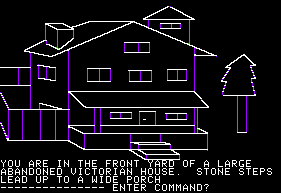
\includegraphics{img/Mystery_House.png}
\caption{The opening scene from Myster House (1980). Source: https://commons.wikimedia.org\cite{wiki:MysteryHouse}}
\label{fig:g}
\end{figure}
\todo{picture is completely off!}

This is where the contenders for the title of the first point-and-click adventure game come into the scene, among those being \textit{Enchanted Scepters}. For many years, this game was thought to have debuted in 1984. However, subsequent investigations revealed that its release likely occurred later, in November 1985. This revelation has shifted the discussion, with \textit{Deja Vu: A Nightmare Begins}, released at least a month earlier, now emerges as a leading candidate for the first true point-and-click adventure game \cite{Pfenning2024}.

The ambiguity surrounding these early releases reflects the gradual evolution of the genre, as developers experimented with interactive storytelling and gameplay mechanics. These pioneering efforts laid the groundwork for the point-and-click adventure games that followed, shaping the genre into the recognizable form that captivated audiences in the years to come.

Point-and-click adventure games experienced their golden age in the late 1980s and early 1990s, with iconic titles such as \textit{The Secret of Monkey Island} (1990), \textit{Beneath a Steel Sky} (1994), and \textit{Myst} (1994) captivating players with their innovative storytelling and puzzle-solving gameplay. However, as the decade progressed, the popularity of the genre waned\cite{Qaffas202022}, with fewer mainstream releases and a shift to niche titles such as the \textit{Nancy Drew} game series.

In recent years, the point-and-click adventure genre has undergone a renaissance. Modern titles such as \textit{Thimbleweed Park} (2017) and \textit{Return to Monkey Island} (2022) have revived interest by paying homage to the retro roots of the genre while incorporating modern design elements. This resurgence has also been fueled by the cinematic storytelling approach pioneered by \textit{Telltale Games}, whose narrative-driven series brought the genre back into the mainstream spotlight.

The renewed interest in point-and-click adventure games highlights their timeless appeal and presents an opportunity for new developers to explore the genre. Building on its rich legacy, aspiring game creators can reimagine and modernize these games for contemporary audiences. This cultural revival underscores the need for accessible development tools to support and sustain the creative evolution of this genre.

\chapter{Important first chapter}
\label{chap:refs}

First chapter usually builds the theoretical background necessary for readers to understand the rest of the thesis. You should summarize and reference a lot of existing literature and research.

You should use the standard \emph{citations}\todo{Use \textbackslash{}emph command like this, to highlight the first occurrence of an important word or term. Reader will notice it, and hopefully remember the importance.}.

\begin{description}
\item[Obtaining bibTeX citation] Go to Google Scholar\footnote{\url{https://scholar.google.com}}\todo{This footnote is an acceptable way to `cite' webpages or URLs. Documents without proper titles, authors and publishers generally do not form citations. For this reason, avoid citations of wikipedia pages.}, find the relevant literature, click the tiny double-quote button below the link, and copy the bibTeX entry.
\item[Saving the citation] Insert the bibTeX entry to the file \texttt{refs.bib}. On the first line of the entry you should see the short reference name --- from Scholar, it usually looks like \texttt{author2015title} --- you will use that to refer to the citation.
\item[Using the citation] Use the \verb|\cite| command to typeset the citation number correctly in the text; a long citation description will be automatically added to the bibliography at the end of the thesis. Always use a non-breakable space before the citing parenthesis to avoid unacceptable line breaks:
\begin{Verbatim}
Trees utilize gravity to invade ye
noble sires~\cite{newton1666apple}.
\end{Verbatim}
\item[Why should I bother with citations at all?] For two main reasons:
\begin{itemize}
\item You do not have to explain everything in the thesis; instead you send the reader to refer to details in some other literature. Use citations to simplify the detailed explanations.
\item If you describe something that already exists without using a citation, the reviewer may think that you \emph{claim} to have invented it. Expectably, they will demand academic correctness, and, from your perspective, being accused of plagiarism is not a good starting point for a successful defense. Use citations to identify the people who invented the ideas that you build upon.
\end{itemize}
\item[How many citations should I use?]
Cite any non-trivial building block or assumption that you use, if it is published in the literature. You do not have to cite trivia, such as the basic definitions taught in the introductory courses.

The rule of thumb is that you should read, understand and briefly review at least around 4 scientific papers. A thesis that contains less than 3 sound citations will spark doubt in reviewers.
\end{description}

There are several main commands for inserting citations, used as follows:
\begin{itemize}
\item \citet{knuth1979tex} described a great system for typesetting theses.
\item We are typesetting this thesis with \LaTeX, which is based on \TeX{} and METAFONT~\cite{knuth1979tex}.
\item \TeX{} was expanded to \LaTeX{} by \citet{lamport1994latex}, hence the name.
\item Revered are the authors of these systems!~\cite{knuth1979tex,lamport1994latex}
\end{itemize}

\section{Some extra assorted hints before you start writing English}

\paragraph{Word order}
Strictly adhere to the English word order rules. The sentences follow a fixed structure with a subject followed by a verb and an object (in this order). Exceptions to this rule must be handled specially, and usually separated by commas.

\paragraph{Sentence structure}
Do not write long sentences. One sentence should contain exactly one fact. Multiple facts should be grouped in a paragraph to communicate one coherent idea. Both the sentences and paragraphs should include various hints about their relation to the other ideas and paragraps. These are typically materialized as adverbs or short sentence parts that clarify the cause--outcome and target--method--result relationship of the sentences in a paragraph. Such `word glue' helps the readers to correctly draw the lines that hold their mental images of your thesis together, and ideally see the big picture of what you were trying to convey right from the first read.

Paragraphs are grouped in labeled sections for a sole purpose of making the navigation in the thesis easier. Do not use the headings as `names for paragraphs' --- the text should make perfect sense even if all headings are removed. If a section of your text contains one paragraph per heading, you might have wanted to write an explicit list instead.

Mind the rules for placing commas:
\begin{itemize}
\item Do not use the comma before subordinate clauses that begin with `that' (like this one). English does not use subordinate clauses as often as Slavic languages because the lack of a suitable word inflection method makes them hard to understand. In scientific English, try to avoid them as much as possible. Ask doubtfully whether each `which' and `when' is necessary --- most of these helper conjunctions can be removed by converting the clause to non-subordinate.

As an usual example, \xxx{\textit{`The sentence, which I wrote, seemed ugly.'}} is perfectly bad; slightly improved by \xxx{\textit{`The sentence that I wrote seemed ugly.'}}, which can be easily reduced to \textit{`The sentence I wrote seemed ugly.'}. A final version with added storytelling value could say \textit{`I wrote a sentence but it seemed ugly.'}
\item Use the \emph{Oxford comma} before `and' and `or' at the end of a longer, comma-separated list of items. Certainly use it to disambiguate any possible mixtures of conjunctions: \textit{`The car is available in red, red and green, and green versions.'} Remember that English `or' is typically understood more like `either this or that, but not both,' and the use of `and` is much more appropriate in cases such as possibility overviews and example listings (like in this sentence).
\item Consider placing extra commas around any parts of the sentence that break the usual word order, especially if they are longer than a single word.
\end{itemize}

\paragraph{Nouns}
Every noun needs a determiner (`a', `the', `my', `some', \dots); the exceptions to this rule, such as non-adjectivized names and indeterminate plural, are relatively scarce. Without a determiner, a noun can be easily mistaken for something completely different, such as an adjective or a verb.

Name all things with appropriate nouns to help both the reader and yourself, and do not hesitate to invent good names and labels for anything that you will refer to more than once. Proper naming will save you a lot of writing effort because you will not have to repeat descriptions such as \xxx{\textit{`the third output of the second benchmarked method of the improved set,'}} instead you may introduce a labeling that will allow you to say just something like \textit{`output M2\textsuperscript{+}-3'}. At the same time, this will reduce the risk that the reader will confuse the object with another one --- for illustration, the long version of the previous example might very easily confuse with the second output of the third method. The same also applies to methods descriptions, algorithms, programs, testing datasets, theorems, use-cases, challenges and other things. As an example, \xxx{\textit{`the algorithm that organizes the potatoes into appropriate buckets'}} shortens nicely as \textit{`the potato bucketer'} and may be labeled as a procedure \textsc{BucketPotatoes()}, and \xxx{\textit{`the issue where the robot crashes into a wall and takes significant time to return to the previous task'}} may be called just \textit{`the crash-recovery lag'}.

\paragraph{Verbs}
Although English can express a whopping 65 base verb tenses and their variants, scientific literature often suppresses this complexity and uses only several basic tenses where the meaning is clearly defined. Typically, you state facts in present simple (\textit{`Theorem 1 proves that Gadget B works as intended.'}), talk about previous work and experiments done in past simple (\textit{`We constructed Gadget B from Gizmo C, which was previously prepared by Tinkerer et al.'}), and identify achieved results in present perfect (\textit{`We have constructed Technology T.'}). Avoid using future tense, except for sections that explicitly describe future work --- as a typical mistake, if you state that the thesis \emph{will} describe something in later chapters, you imply that the description is not present there yet.

Do not write sentences in passive voice, unless you explicitly need to highlight that something has passively subjected itself to an action. Active voice is more preferable in the theses because it clearly highlights the actors and their contributions --- typically, \textit{`you did it'} instead of \textit{`it was done'} by a mysterious entity, which the reviewers rarely envision as yourself. Writing in active voice additionally benefits the explanation of complex processes: There, the word order forces you to identify the acting subject as the first word in the sentence, which further disambiguates how the individual process parts are triggered and ordered.

Try to avoid overusing gerunds (verbs that end with `-ing'). It is convenient to write shorter sentences by using gerunds as adjectives, but these are typically quite hard to understand because the readers may easily confuse the intended adjectives with verbs. If your sentence contains two gerunds close to each other, it may need a rewrite.

\paragraph{Scientific writing resources}
Consult the book by \citet{glasman2010science} for more useful details and recommended terminology for writing about the scientific research. Very pragmatically, the book by \citet{sparling1989english} describes many common mistakes that Czech and Slovak (and generally Slavic) writers make when writing English.

\chapter{Important second chapter}
\label{chap:refs}





\chapter{Results and discussion}

You should have a separate chapter for presenting your results (generated by the stuff described previously, in our case in \cref{chap:math}). Remember that your work needs to be validated rigorously, and no one will believe you if you just say that `it worked well for you'.

Instead, try some of the following:
\begin{itemize}
\item State a hypothesis and prove it statistically
\item Show plots with measurements that you did to prove your results (e.g. speedup). Use either \texttt{R} and \texttt{ggplot}, or Python with \texttt{matplotlib} to generate the plots.\footnote{Honestly, the plots from \texttt{ggplot} look \underline{much} better.} Save them as PDF to avoid printing pixels (as in \cref{fig:f}).
\item Compare with other similar software/theses/authors/results, if possible
\item Show example source code (e.g. for demonstrating how easily your results can be used)
\item Include a `toy problem' for demonstrating the basic functionality of your approach and detail all important properties and results on that
\item Include clear pictures of `inputs' and `outputs' of all your algorithms, if applicable
\end{itemize}

\begin{figure}
\centering
\includegraphics[width=.6\linewidth]{img/ukazka-obr01.pdf}
\caption{This caption is a friendly reminder to never insert figures ``in text,'' without a floating environment, unless explicitly needed for maintaining the text flow (e.g., the figure is small and developing with the text, like some of the centered equations, as in \cref{thm:y}). All figures \emph{must} be referenced by number from the text (so that the readers can find them when they read the text) and properly captioned (so that the readers can interpret the figure even if they look at it before reading the text --- reviewers love to do that).}
\label{fig:f}
\end{figure}

It is sometimes convenient (even recommended by some journals, including Cell) to name the results sub-sections so that they state what exactly has been achieved. Examples follow.

\section{SuperProgram is faster than OldAlgorithm}
\subsection{Scalability estimation}
\subsection{Precision of the results}
\section{Weird theorem is proven by induction}
\section{Amount of code reduced by CodeRedTool}
\subsection{Example}
\subsection{Performance on real codebases}
\section{\sloppy NeuroticHelper improves neural network learning}

\section{Graphics and figure quality}

No matter how great the text content of your thesis is, the pictures will always catch the attention first. This creates the very important first impression of the thesis contents and general quality. Crucially, that also decides whether the thesis is later read with joy, or carefully examined with suspicion.

Preparing your thesis in a way such that this first impression gets communicated smoothly and precisely helps both the reviewer and you: the reviewer will not have a hard time understanding what exactly you wanted to convey, and you will get a better grade.

Making the graphics `work for you' involves doing some extra work that is often unexpected. At the same time, you will need to fit into graphics quality constraints and guidelines that are rarely understood before you actually see a bad example. As a rule of thumb, you should allocate at least the same amount of time and effort for making the figures look good as you would for writing, editing and correcting the same page area of paragraph text.

\subsection{Visualize all important ideas}
The set of figures in your thesis should be comprehensive and complete. For all important ideas, constructions, complicated setups and results there should be a visualization that the reader can refer to in case the text does not paint the `mental image' sufficiently well. At the bare minimum, you should have at least 3 figures (roughly corresponding to the 3 chapters) that clearly and unambiguously show:
\begin{enumerate}
\item the context of the problem you are solving, optionally with e.g.~question marks and exclamation marks placed to highlight the problems and research questions
\item the overall architecture of your solution (usually as a diagram with arrows, such as in \cref{fig:schema}, ideally with tiny toy examples of the inputs and outputs of each box),
\item the advancement or the distinctive property of your solution, usually in a benchmark plot, or as a clear demonstration and comparison of your results.
\end{enumerate}

\subsection{Make the figures comprehensible}
The figures should be easily comprehensible. Surprisingly, that requires you to follow some common ``standards'' in figure design and processing. People are often used to a certain form of the visualizations, and (unless you have a very good reason) deviating from the standard is going to make the comprehension much more complicated. The common standards include the following:
\begin{itemize}
  \item caption everything correctly, place the caption at an expectable position
  \item systematically label the plots with `main' titles (usually in boldface, above the plot), plot axes, axis units and ticks, and legends
  \item lay out the diagrams systematically, ideally follow a structure of a bottom-up tree, a left-to-right pipeline, a top-down layered architecture, or a center-to-borders mindmap
  \item {use colors that convey the required information correctly \par\footnotesize Although many people carry some intuition for color use, achieving a really correct utilization of colors is often very hard without previous experience in color science and typesetting. Always remember that everyone perceives color hues differently, therefore the best distinction between the colors is done by varying lightness of the graphics elements (i.e., separating the data by dark vs.~light) rather than by using hues (i.e., forcing people to guess which one of salmon and olive colors means ``better''). Almost 10\% of the population have their vision impaired by some form of color vision deficiency, most frequently by deuteranomaly that prevents interpretation of even the most `obvious' hue differences, such as green vs.~red. Finally, printed colors look surprisingly different from the on-screen colors. You can prevent much of these problems by using standardized palettes and well-tested color gradients, such as the ones from ColorBrewer\footnote{\url{https://colorbrewer2.org}} and ViridisLite\footnote{\url{https://sjmgarnier.github.io/viridisLite/}}. Check if your pictures still look good if converted to greyscale, and use a color deficiency simulator to check how the colors are perceived with deuteranomaly.}
\end{itemize}

Avoid large areas of over-saturated and dark colors:
\begin{itemize}
  \item under no circumstances use dark backgrounds for any graphical elements, such as diagram boxes and tables --- use very light, slightly desaturated colors instead
  \item avoid using figures that contain lots of dark color (as a common example, heatmaps rendered with the `magma' color palette often look like huge black slabs that are visible even through the paper sheet, thus making a dark smudge on the neighboring page)
  \item increase the brightness of any photos to match the average brightness of the text around the figure
\end{itemize}

Remember to test your figures on other people --- usually, just asking `What do you think the figure should show?' can help you debug many mistakes in your graphics. If they think that the figure says something different than what you planned, then most likely it is your figure what is wrong, not the understanding of others.

Finally, there are many magnificent resources that help you arrange your graphics correctly. The two books by Tufte~\cite{tufte1990envisioning,tufte1983visual} are arguably classics in the area. Additionally, you may find many interesting resources to help you with technical aspects of plotting, such as the \texttt{ggplot}-style `Fundamentals' book by~\citet{wilke2019fundamentals}, and a wonderful manual for the TikZ/PGF graphics system by~\citet{tantau2015tikz} that will help you draw high-quality diagrams (like the one in~\cref{fig:schema}).

\section{What is a discussion?}
After you present the results and show that your contributions work, it is important to \emph{interpret} them, showing what they mean in the wider context of the thesis topic, for the researchers who work in the area, and for the more general public, such as for the users.

Separate discussion sections are therefore common in life sciences where some ambiguity in result interpretation is common, and the carefully developed intuition about the wider context is sometimes the only thing that the authors have. Exact sciences and mathematicians do not need to use the discussion sections as often. Despite of that, it is nice to position your output into the previously existing environment, answering:
\begin{itemize}
\item What is the potential application of the result?
\item Does the result solve a problem that other people encountered?
\item Did the results point to any new (surprising) facts?
\item How (and why) is the approach you chose different from what the others have done previously?
\item Why is the result important for your future work (or work of anyone other)?
\item Can the results be used to replace (and improve) anything that is used currently?
\end{itemize}

If you do not know the answers, you may want to ask the supervisor. Also, do not worry if the discussion section is half-empty or completely pointless; you may remove it completely without much consequence. It is just a bachelor thesis, not a world-saving avenger thesis.

\chapter{Results and discussion}

You should have a separate chapter for presenting your results (generated by the stuff described previously, in our case in \cref{chap:math}). Remember that your work needs to be validated rigorously, and no one will believe you if you just say that `it worked well for you'.

Instead, try some of the following:
\begin{itemize}
\item State a hypothesis and prove it statistically
\item Show plots with measurements that you did to prove your results (e.g. speedup). Use either \texttt{R} and \texttt{ggplot}, or Python with \texttt{matplotlib} to generate the plots.\footnote{Honestly, the plots from \texttt{ggplot} look \underline{much} better.} Save them as PDF to avoid printing pixels (as in \cref{fig:f}).
\item Compare with other similar software/theses/authors/results, if possible
\item Show example source code (e.g. for demonstrating how easily your results can be used)
\item Include a `toy problem' for demonstrating the basic functionality of your approach and detail all important properties and results on that
\item Include clear pictures of `inputs' and `outputs' of all your algorithms, if applicable
\end{itemize}

\begin{figure}
\centering
\includegraphics[width=.6\linewidth]{img/ukazka-obr01.pdf}
\caption{This caption is a friendly reminder to never insert figures ``in text,'' without a floating environment, unless explicitly needed for maintaining the text flow (e.g., the figure is small and developing with the text, like some of the centered equations, as in \cref{thm:y}). All figures \emph{must} be referenced by number from the text (so that the readers can find them when they read the text) and properly captioned (so that the readers can interpret the figure even if they look at it before reading the text --- reviewers love to do that).}
\label{fig:f}
\end{figure}

It is sometimes convenient (even recommended by some journals, including Cell) to name the results sub-sections so that they state what exactly has been achieved. Examples follow.

\section{SuperProgram is faster than OldAlgorithm}
\subsection{Scalability estimation}
\subsection{Precision of the results}
\section{Weird theorem is proven by induction}
\section{Amount of code reduced by CodeRedTool}
\subsection{Example}
\subsection{Performance on real codebases}
\section{\sloppy NeuroticHelper improves neural network learning}

\section{Graphics and figure quality}

No matter how great the text content of your thesis is, the pictures will always catch the attention first. This creates the very important first impression of the thesis contents and general quality. Crucially, that also decides whether the thesis is later read with joy, or carefully examined with suspicion.

Preparing your thesis in a way such that this first impression gets communicated smoothly and precisely helps both the reviewer and you: the reviewer will not have a hard time understanding what exactly you wanted to convey, and you will get a better grade.

Making the graphics `work for you' involves doing some extra work that is often unexpected. At the same time, you will need to fit into graphics quality constraints and guidelines that are rarely understood before you actually see a bad example. As a rule of thumb, you should allocate at least the same amount of time and effort for making the figures look good as you would for writing, editing and correcting the same page area of paragraph text.

\subsection{Visualize all important ideas}
The set of figures in your thesis should be comprehensive and complete. For all important ideas, constructions, complicated setups and results there should be a visualization that the reader can refer to in case the text does not paint the `mental image' sufficiently well. At the bare minimum, you should have at least 3 figures (roughly corresponding to the 3 chapters) that clearly and unambiguously show:
\begin{enumerate}
\item the context of the problem you are solving, optionally with e.g.~question marks and exclamation marks placed to highlight the problems and research questions
\item the overall architecture of your solution (usually as a diagram with arrows, such as in \cref{fig:schema}, ideally with tiny toy examples of the inputs and outputs of each box),
\item the advancement or the distinctive property of your solution, usually in a benchmark plot, or as a clear demonstration and comparison of your results.
\end{enumerate}

\subsection{Make the figures comprehensible}
The figures should be easily comprehensible. Surprisingly, that requires you to follow some common ``standards'' in figure design and processing. People are often used to a certain form of the visualizations, and (unless you have a very good reason) deviating from the standard is going to make the comprehension much more complicated. The common standards include the following:
\begin{itemize}
  \item caption everything correctly, place the caption at an expectable position
  \item systematically label the plots with `main' titles (usually in boldface, above the plot), plot axes, axis units and ticks, and legends
  \item lay out the diagrams systematically, ideally follow a structure of a bottom-up tree, a left-to-right pipeline, a top-down layered architecture, or a center-to-borders mindmap
  \item {use colors that convey the required information correctly \par\footnotesize Although many people carry some intuition for color use, achieving a really correct utilization of colors is often very hard without previous experience in color science and typesetting. Always remember that everyone perceives color hues differently, therefore the best distinction between the colors is done by varying lightness of the graphics elements (i.e., separating the data by dark vs.~light) rather than by using hues (i.e., forcing people to guess which one of salmon and olive colors means ``better''). Almost 10\% of the population have their vision impaired by some form of color vision deficiency, most frequently by deuteranomaly that prevents interpretation of even the most `obvious' hue differences, such as green vs.~red. Finally, printed colors look surprisingly different from the on-screen colors. You can prevent much of these problems by using standardized palettes and well-tested color gradients, such as the ones from ColorBrewer\footnote{\url{https://colorbrewer2.org}} and ViridisLite\footnote{\url{https://sjmgarnier.github.io/viridisLite/}}. Check if your pictures still look good if converted to greyscale, and use a color deficiency simulator to check how the colors are perceived with deuteranomaly.}
\end{itemize}

Avoid large areas of over-saturated and dark colors:
\begin{itemize}
  \item under no circumstances use dark backgrounds for any graphical elements, such as diagram boxes and tables --- use very light, slightly desaturated colors instead
  \item avoid using figures that contain lots of dark color (as a common example, heatmaps rendered with the `magma' color palette often look like huge black slabs that are visible even through the paper sheet, thus making a dark smudge on the neighboring page)
  \item increase the brightness of any photos to match the average brightness of the text around the figure
\end{itemize}

Remember to test your figures on other people --- usually, just asking `What do you think the figure should show?' can help you debug many mistakes in your graphics. If they think that the figure says something different than what you planned, then most likely it is your figure what is wrong, not the understanding of others.

Finally, there are many magnificent resources that help you arrange your graphics correctly. The two books by Tufte~\cite{tufte1990envisioning,tufte1983visual} are arguably classics in the area. Additionally, you may find many interesting resources to help you with technical aspects of plotting, such as the \texttt{ggplot}-style `Fundamentals' book by~\citet{wilke2019fundamentals}, and a wonderful manual for the TikZ/PGF graphics system by~\citet{tantau2015tikz} that will help you draw high-quality diagrams (like the one in~\cref{fig:schema}).

\section{What is a discussion?}
After you present the results and show that your contributions work, it is important to \emph{interpret} them, showing what they mean in the wider context of the thesis topic, for the researchers who work in the area, and for the more general public, such as for the users.

Separate discussion sections are therefore common in life sciences where some ambiguity in result interpretation is common, and the carefully developed intuition about the wider context is sometimes the only thing that the authors have. Exact sciences and mathematicians do not need to use the discussion sections as often. Despite of that, it is nice to position your output into the previously existing environment, answering:
\begin{itemize}
\item What is the potential application of the result?
\item Does the result solve a problem that other people encountered?
\item Did the results point to any new (surprising) facts?
\item How (and why) is the approach you chose different from what the others have done previously?
\item Why is the result important for your future work (or work of anyone other)?
\item Can the results be used to replace (and improve) anything that is used currently?
\end{itemize}

If you do not know the answers, you may want to ask the supervisor. Also, do not worry if the discussion section is half-empty or completely pointless; you may remove it completely without much consequence. It is just a bachelor thesis, not a world-saving avenger thesis.



\chapwithtoc{Conclusion}

In the conclusion, you should summarize what was achieved by the thesis. In a few paragraphs, try to answer the following:
\begin{itemize}
\item Was the problem stated in the introduction solved? (Ideally include a list of successfully achieved goals.)
\item What is the quality of the result? Is the problem solved for good and the mankind does not need to ever think about it again, or just partially improved upon? (Is the incompleteness caused by overwhelming problem complexity that would be out of thesis scope\todo{This is quite common.}, or any theoretical reasons, such as computational hardness?)
\item Does the result have any practical applications that improve upon something realistic?
\item Is there any good future development or research direction that could further improve the results of this thesis? (This is often summarized in a separate subsection called `Future work'.)
\end{itemize}

\include{bibliography}

\appendix
\include{howto}

% if your attachments are complicated, describe them in a separate appendix
%\include{attachments}

\openright
\end{document}
